\documentclass[fleqn]{jbook}
\usepackage{physpub}

\begin{document}

\begin{question}{専攻 問題8}{}

\begin{subquestions}
\unitlength=1ex
\SubQuestion
  蛋白質は熱や酸によりこわれた天然状態から変性状態に変る。この構造
  変化について蛋白質の熱力学を考えよう。\\
  蛋白質の安定性は上記2つの状態の自由エネルギー差を用いて議論され、
  通常記号
  $\IDelta G^u\ (G^{\mbox{\small 変性}}-G^{\mbox{\small 天然}})$
  で表される。$\IDelta G^u$は熱の出入りを表すエンタルピー$\IDelta H^u$
  と分子の無秩序を表すエントロピー $\IDelta S^u$の2項を用いて次の式で
  表現される。
%
  \begin{equation}
    \IDelta G^u = \IDelta H^u -T \IDelta S^u \eqname{Q1}
  \end{equation}
%
  ところで、$\IDelta G^u,\,\IDelta S^u$の温度依存性は以下のように
  カロリメトリー測定より求まる。
%
  \begin{eqnarray}
    \IDelta H^u &=& \IDelta H_m + \int_{T_m}^{T}\IDelta C_p \d{T} 
    = \framebox(20,2)[c]{a}  \eqname{Q2} \\
    \IDelta S^u &=& \frac{\IDelta H_m }{T_m}
    + \int_{T_m}^{T}\IDelta C_p \d{(\ln{T})}
    = \framebox(20,2)[c]{b}  \eqname{Q3}
  \end{eqnarray}
%
  ここで、$T_m$と$\IDelta H_m$は変性中点の温度(変性温度)と変性の潛熱
  である。また、$\IDelta C_p$は2つの状態の比熱の差で温度によらない
  定数とする。式\eqhref{Q1},\eqhref{Q2},\eqhref{Q3}より、
  $\IDelta G^u$の温度依存性は最終的に下の式で与えられる。
%
  \[ \IDelta G^u = \framebox(20,2)[c]{c} \]
%

\SubQuestion
  蛋白質の一つであるリゾチームのカロリメトリー測定からpH7で以下の
  値が得られた。\\
%
  $\IDelta H_m = 100 \Unit{kcal/mol},\quad%
   \IDelta C_p = 2.3 \Unit{kcal/mol \cdot K},\quad%
  T_m = 57\degC$\\
%
  この値をもとに $\IDelta G^u,\,\IDelta H^u,\,\IDelta S^u$
  の温度変化を図示せよ。\\
  この図よりリゾチームの最安定状態の温度\framebox(10,2)[c]{d}を
  導け。またこの温度で$\IDelta S^u = 0$となることを導け。

\SubQuestion
  物質は低温で安定だが、蛋白質は高温のみならず低温で不安定となる
  (低温変性)。この理由について考察しよう。\\
%
  $\IDelta G^u,\,\IDelta H^u,\,\IDelta S^u$は無水状態(真空中)の純粋に
  蛋白質構造の寄与(添字をcで表す)と蛋白質と水との相互作用の項(水和
  エネルギー、添字をhで表す)の2項に分解される。
%
  \begin{eqnarray}
    \IDelta G^u &=& \IDelta G^u_c + \IDelta G^u_h \eqname{Q4} \\
    \IDelta H^u &=& \IDelta H^u_c + \IDelta H^u_h \eqname{Q5} \\
    \IDelta S^u &=& \IDelta S^u_c + \IDelta S^u_h \eqname{Q6}
  \end{eqnarray}
%
  このうち蛋白質構造由来の項 $\IDelta H^u_c,\,\IDelta S^u_c$
  の温度依存性は小さい。この値を一定と考えると、
  $\IDelta G^u_c = 0 $となる温度、すなわち真空中の変性温度は一点で
  定まり、低温変性はあり得ない。たとえば、
  $\IDelta H^u_c = 870  \Unit{kcal/mol}$,\\
  $\IDelta S^u_c = 1700 \Unit{kcal/mol \cdot K}$
  のとき真空中の変性温度は\framebox(10,2)[c]{e}と見積もられる。
  水中では {\bf 2}の問題に見られるように$\IDelta G^u = 0 $となる点が
  2つある。従ってこれは$\IDelta H^u_c $,$\IDelta S^u_c $ではなく
  $\IDelta H^u_h $,$\IDelta S^u_h $の水和エネルギーにその起源があると
  考えなければならない。

\SubQuestion
  水との相互作用エネルギー(水和エネルギー)は以下で与えられる。
%
  \begin{eqnarray}
    \IDelta H^u_h &=&%
      \IDelta H^u_h (T_0) + \int_{T_0}^{T}\IDelta C_p \d{T}%
      \eqname{Q7}\\
    \IDelta S^u_h &=&%
      \IDelta S^u_h (T_0) + \int_{T_0}^{T}\IDelta C_p \d{(\ln{T})}
      \eqname{Q8}
  \end{eqnarray}
%
  ここでは$T_0$は基準温度、例えば$25\degC$。
%
  \begin{eqnarray}
    \IDelta H^u_h (T_0) &=&
      h_1(A^D_1 - A^N_1) + h_2(A^D_2 - A^N_2)  \eqname{Q9}  \\
    \IDelta S^u_h (T_0) &=&
      s_1(A^D_1 - A^N_1) + s_2(A^D_2 - A^N_2)  \eqname{Q10} \\
    \IDelta G^u_h (T_0) &=&
     {\rm g}_1(A^D_1 - A^N_1) + {\rm g}_2(A^D_2 - A^N_2) \eqname{Q11}
  \end{eqnarray}
%
  ここで$h_1,\,s_1,\,g_1$は極性基のそして$h_2,\,s_2,\,{\rm g}_2$
  は非極性基の水和の熱力学パラメータである。$A^D_1,\,A^N_1$は
  それぞれ水と接する極性基の変性状態と天然状態における総数である。
  非極性基も同様に定義する。\\
  水和の熱エネルギーは表のように与えられる。\\
%
  \parbox[t]{82mm}{
  水和の力学的パラメーター\\
%
  \begin{tabular}{rrrr} \hline
             & h & s & g \\
    基       & (kcal/mol) & (cal/mol$\cdot $K) & (kcal/mol) \\ \hline
    極性基   & $-20$ & $-40$ & $-8$ \\
    非極性基 & $-13$ & $-40$ & $-1$ \\ \hline
  \end{tabular}\\
  }\parbox[t]{75mm}{\vspace*{-10mm}
  \begin{center}
    水和量変化の模式図\\
    \mbox{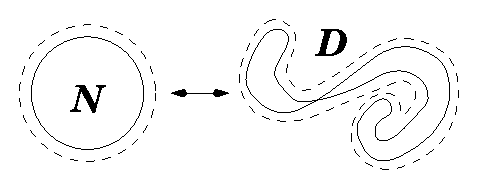
\includegraphics[clip]{1996phy8-1.eps}}
  \end{center}}\\
%
  式\eqhref{Q9}〜\eqhref{Q11}と上表を用いると水和に伴う、各熱力学量は
  蛋白質の構造変化(上図参照)が分かると自動的に求まる。まず
  $\IDelta G^u_h (T_0),\IDelta S^u_h (T_0)$が求まる。次に実験量
  $\IDelta C_p $を用いて式\eqhref{Q7},\eqhref{Q8}より温度変化がわかる。
  その結果が次の図に与えられている。
%
  \begin{center}
    \mbox{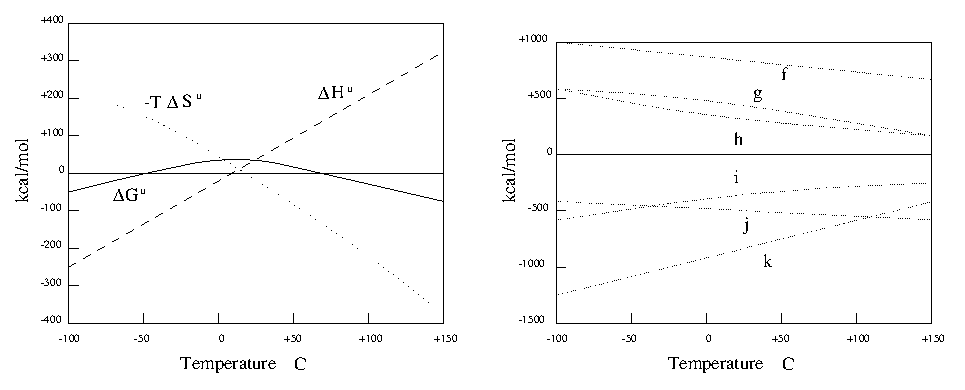
\includegraphics[clip]{1996phy8-2.eps}}
  \end{center}
%
  式\eqhref{Q4}〜\eqhref{Q6}の右辺に表れた6個の熱力学量が上の右の図
  の中の曲線のどれに対応するか示せ。ただし上図では\\
  $\IDelta S^u_c,\,\IDelta S^u_h (T_0)$は
  $-T \IDelta S^u_c,~-T \IDelta S^u_h (T_0)$の形で表示されている。

\SubQuestion
  以上の考察から低温変性の起源について論ぜよ。

\end{subquestions}

\end{question}
\begin{answer}{専攻 問題8}{}

\begin{subanswers}
\SubAnswer
  \vspace*{-5mm}
  \begin{eqnarray*}
  \IDelta H^u &=&%
     \IDelta H_m + \int_{T_m}^{T}\IDelta C_p \d{T}  
     = \IDelta H_m + \IDelta C_p(T-T_m)\\
  \IDelta S^u &=&%
    \frac{\IDelta H_m}{T_m} + \int_{T_m}^{T}\IDelta C_p \d{(\ln{T})}
    = \frac{\IDelta H_m }{T_m} + \IDelta C_p \ln{\frac{T}{T_m}}\\
  \IDelta G^u &=&%
    \IDelta H^u -T \IDelta S^u%
    = \IDelta H_m \left( 1- \frac{T}{T_m} \right)%
    + \IDelta C_p %
      \left\{ \left(T-T_m \right) - T {\rm ln}\frac{T}{T_m} \right\}%
  \end{eqnarray*}

\SubAnswer
  $\IDelta G^u,\,\IDelta H^u,\,\IDelta S^u$の温度変化は下図の通り。
%
  \begin{center}
    \mbox{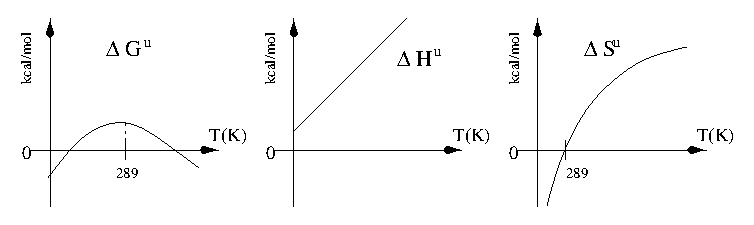
\includegraphics[clip]{1996phy8-3.eps}}
  \end{center}
%
  最も安定になるのは $\tDeriver{(\IDelta G^u)}{T} = 0 $
  のときの温度である。
%
  \begin{eqnarray*}
    \Deriver{(\IDelta G^u)}{T}%
    &=& \Deriver{}{T}\left( \IDelta H^u -T\IDelta S^u \right)%
     =  \Deriver{(\IDelta H^u)}{T}- \IDelta S^u%
        - T \Deriver{(\IDelta S^u)}{T} \\
    &=& \IDelta C_p - \IDelta S^u%
        - T \Deriver{(\ln{T})}{T}\Deriver{}{(\ln{T})}%
        \left( \frac{\IDelta H_m}{T_m}
        + \int \IDelta C_p d(\ln{T}) \right) \\
    &=& \IDelta C_p - \IDelta S^u - \IDelta C_p 
     =  - \IDelta S^u
  \end{eqnarray*}
%
  よって $\IDelta S^u =0$ となる $289\Unit{K}$で最安定。



\SubAnswer
  \[ \IDelta G^u = \IDelta H^u_c + \IDelta H^u_h
     - T(\IDelta S^u_c + \IDelta S^u_h )
     = (\IDelta H^u_c - T \IDelta S^u_c )
     +(\IDelta H^u_h - T \IDelta S^u_h ) \]
%
  真空中だから水との相互作用の項を無視し、
%
  \[ \IDelta G^u = \IDelta H^u_c - T \IDelta S^u_c 
     = 870 - 1.7 \times T \]
%
  よって真空中の変性温度は$\IDelta G^u =0$から$T=512\Unit{K}$
  この一つのみ。

\SubAnswer
  自然状態のタンパク質は、水と接する外側に極性基が、内側に非極性基が
  あるので、
%
  \[ (A^D_1 - A^N_1) > (A^D_2 - A^N_2)  \]
%
  となる。また、純粋にタンパク質構造に寄与する項の温度変化は小さく、
  特徴があまりないと考えられる。よって、まずグラフより水との相互作用
  の項と考える。結果は次のようになる。
%
  \[ \begin{array}{rcll}
     \IDelta H^u_h & \cdots & {\bf j} &
   \mbox{$\IDelta H^u$のグラフのように直線的に右上がりなのはこれだけ}\\
   -T\IDelta S^u_h & \cdots & {\bf g} &
   \mbox{$-T\IDelta S^u$ のグラフより}\\
     \IDelta G^u_h & \cdots & {\bf i} &
   \mbox{$\IDelta G^u_h = \IDelta H^u_h - T \IDelta S^u_h$より}\\
     \IDelta H^u_c & \cdots & {\bf f} &\\
   -T\IDelta S^u_c & \cdots & {\bf k} &\\
     \IDelta G^u_c & \cdots & {\bf h} &
  \end{array} \]

\SubAnswer
  低温変性の起源は水和エネルギーであり、各タンパク質により異なる
  $ \IDelta C_p$や、自然状態と変性状態での水と接する極性・非極性基の
  差が変化することにより、変性温度が変化する。

\end{subanswers}

\end{answer}


\end{document}
